%!TEX root = ../swiatlow_thesis.tex
\label{chapter:color}
\section{Motivation}

What does it mean to see color?

In terms of the color we experience on a day-to-day basis, it means that our eyes (particle detectors in their own right!) respond differently to photons with different energy (that is, different wavelengths). In terms of color at the LHC-- an aspect of the strong nuclear force now, instead of the electromagnetic-- things are much more muddled. Asymptotic freedom and the process of hadronization mean that the particles observed by the LHC detectors are not actually colored themselves-- and so unlike retinas, which measure energy directly, color at the LHC is much less direct.

The first question to ask, when considering measuring color at the LHC, is what potential \textit{measurable} effects color can have, even if the color charge itself is not directly accessible. After all-- $SU(3)_C$ singlets ($W$, $Z$, $\ell$ particles), triplets ($q$ of all types), and octets ($g$) exist: surely there must be some differences between these states. Certainly, seeing red-blue-green is not particularly useful-- there's no consequential differences between a red quark and a green quark. But, seeing the difference between an octet and a singlet might indeed be useful: gluon octets, for example, can be backgrounds to signal singlets. Additionally, the magntitude of the color charge-- in analogy to the magnitude of the electric charge-- might be useful: different types of particles have different  charges (0 for singlets, $1/3$ for triplets, $4/3$ for octets). \editnote{are these numbers correct? $C/A$}

The first evidence of color at a particle collider was observed by the JADE experiment at PETRA-- in a process very familiar to the studies of Section~\ref{jet-reconstruction:qg:validation}. At PETRA, it was observed that the third leading jet (ordered in $p$) in tri-jet events had a \textit{broader} distribution of energy (comparing the distance of particles to the center of the jet axis) than that of the leading two jets: this was interepreted as evidence for the third jet being more likely to a gluon, whie the leading two were quarks~\cite{Bartel:1983ii}. This is exactly the same effect seen by ATLAS in Section~\ref{jet-reconstruction:qg:validation}, and is directly related to the magnitude of the color charge: the larger color charge for gluons implies that they fragment ``more,'' and consequentially have a higher multiplicity and less collimated shower. This first observation from PETRA sets the stage for color will be observed in other experiments: often it is not a direct effect on the 4-momentum of a jet, but is instead a property of the jet \textit{shape}. 

A similar property, also first measured by PETRA but now explored by a variety of analyses at PEP, the Tevatron, and the LHC, is called \textit{color coherence}: this refers to the interaction of colored particles during the showering/fragmentation phase of an event, and implies that the angular distribution of jets should be somewhat different from the non-connected expectation. Many experiments have observed effects related to color coherence, at both $e^+/e^-$ and hadron-hadron colliders, in multi-jet events.~\cite{tasso,pep,PhysRevLett54270,PhysRevLett57945,PhysRevLett571398,PhysRevD.50.5562,Abbott:1997bk,Chatrchyan:2013fha}. In this type of analysis, color is sometimes measured with jet shapes, and sometimes indirectly via the push/pull of the jet axis away/towards some other jet.

% look into these papers
% bah compiling errors
Colliders operating above the $W/Z$ mass scale can produce the vector bosons, and as these are color singlets, they provide an interesting testing ground for the measurement of color. These can be a testground for further color coherence studies, as studied by the Tevatron by measuring the calorimeter activity around leptonic $W$'s and jets~\cite{Abbott:1999cu}.  L3 and DELPHI, in turn, studied the energy between $W$ bosons in $WW$ events, comparing pairs of jets from the same or different $W$, and observed that different color flow models predicted different behavior, in a process referred to as \textit{color reconnection}~\cite{Achard:2003pe,Abdallah:2006uq}. In these studies, $W$ bosons were used as test samples to study color, usually by looking outside of the jet for additional radiation: color was visible not as a property of the jet, but of the environment surrounding it.

Most of these measurements have been sensitive to the presence of color-- indeed, the seminal JADE measurement is even principle to the magntitude of the color charge-- but most of them are used to constrain color \textit{models}, and not determine the actual color properties of objects. That is to say, these measurements all help tune MC generators and shower models to more accurately reproduce the effects of hadronization and the residual effects of color, but none of them have measured the actual color representation of the $W$, for example. While it is clear from leptonic helicity measurements and $W$+jets production cross-sections that the $W$-boson is a color singlet, the hadronic decays of a $W$ have not been used to \textit{directly} measure the color type: the most direct way of \textit{seeing color} at colliders has not been performed.

Figure~\ref{fig:detector:schematic} gives an example of the color flow in the SM on the left hand side: this blue line connecting the $W$-daughter quarks is the color connection between the two jets, and is determined by the color type of the $W$: because it is a singlet, it cannot carry a color line itself, and so colored objects decaying from it must be connected (via blue/anti-blue, for example). On the right side is an example of a hypothetical alternative model, where the $W$ acts as a color octet: then, it is able to carry \textit{two} colors, and the $W$-daughter quarks do not share a color connection. The effect for this connecting color line is often referred to as \textit{color flow}. Does the blue color line in this figure exist? How can we tell?

%%%%%%%%%%%%%%%%

\begin{figure}
\centering
\includegraphics[width=0.7\textwidth]{paper/schematic.pdf}
\label{fig:color:motivation:schematic}
\caption{An example of the color flow in SM $t\bar{t}$ events on the left, and a hypothetical exotic model where the $W$ is an octet on the right.}
\end{figure}

%%%%%%%%%%%%%%%%  

This question is not just academic: telling the difference between a singlet and an octet can already be useful in LHC searches. For example, the Higgs boson has not yet been observed in its decay to $b$-quarks: as a singlet, it should have a different color flow from that of the main gluon backgrounds. Likewise, if a new particle is discovered in a dijet resonance, it will be immediately important to characterize its color representation: measuring the color flow, in a similar way to the schematic of Figure~\ref{fig:detector:schematic}, will be critical. 

\section{The Pull Angle}

What we have learned so far from previous color measurements is that two basic categories of information are useful in seeing color related effects:
%
\begin{enumerate}
\item Energy distributions inside, or surrounding, jets
\item Orientation of jet axes, and angular kinematics 
\end{enumerate}
%
One recently developed variable, the \textit{jet pull}, combines both of these types of information~\cite{Gallicchio:2010sw}. The variable composes a vector of a \pt and radial distance weighted sum over constituents of a jet and determines the oriention of this vector in relation to other jets, thereby combining the structural information about the jet with the broader context of the event (in a strategy sometimes referred to as jet superstructure). The D0 and CMS collaborations, as well as theorists, have used this variable as a part of multivariate analyses to improve sensitivity to Higgs decays to b-quarks already.~\cite{D0higgs,CMShiggspap,CMShiggspap2}. D0 also attempted a measurement of the color flow using the pull in top quark decays, comparing reconstructed data events to templates of the pull composed using singlet and octet $W$-boson models; the result, however, was strongly statistically limited and not able to distinguish.

The first step in measuring color flow with pull is to construct for a jet its \textit{pull vector}, defined as:
%
\begin{align}
\vec{v} = \sum_{i\in J} \frac{p_T^i |r_i|}{p_T^{J}}\vec{r}_i,
\end{align}
%
where $i$ iterates over elements (topo-clusters or tracks or truth particles) associated to some jet $J$, $\vec{r}_i = (\Delta y_i,\Delta\phi_i)$ (i.e. the vector composed of the difference in rapidity and azimuthal angle between the element and the jet axis). The pull vector encodes the substructure information related to the color flow of the jet: the vector points in the direction that the jet is \textit{leaning} in some sense. By itself, this information is not particularly interesting; what makes it useful is its relation to other jets. Given a pull vector composed for a jet $J_1$, the \textit{jet pull angle} $\theta_P(J_1, J_2)$is the opening angle between $\vec{v}_1$ and a jet $J_2$ in $(\Delta y,\Delta\phi)$ space~\cite{Gallicchio:2010sw}. Figure~\ref{fig:color:motivation:pull} is a sketch which demonstrates the various components of this variable: $J_1$ sits at the origin of the $(\Delta y,\Delta\phi)$ coordinate system, and its constituents (the small circles) are used to construct the pull vector $\vec{v}$; the vector between $J_1$ and $J_2$ is also drawn, and the angle between these two vectors is called $\theta_P$, the observable of interest. This schematic also points out that there are two ways for a constituent to contribute strongly to the pull vector: either it has large $\pt$ or a large $r_i$, or both. In a color connected pair of jets-- that is, a pair of jets with a color line connecting them as in the left of Figure~\ref{fig:detector:schematic}-- it is expected that the jets should lean \textit{towards each other}: their energy should be oriented between them, and the pull angle should tend to 0. On the other hand, un-connected jets-- such as the right side of Figure~\ref{fig:detector:schematic}-- should have no preferred orientation, and so the pull angle is expected to be essentially isotropically distributed. Note that while in principle $\theta_P$ ranges from $-\pi$ to $\pi$, the distribution should  be symmetric, and so in all of the following analysis we define $\theta_P$ as the absolute value of the pull angle.




\begin{figure}[h!]
 \centering
		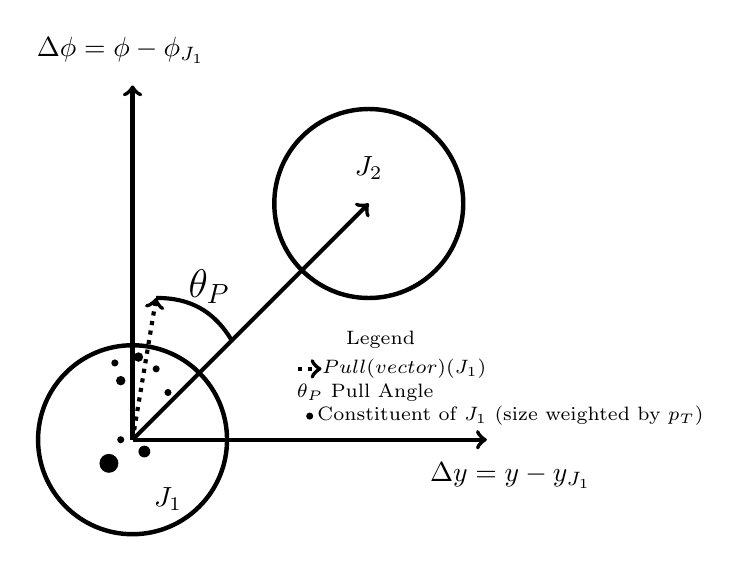
\begin{tikzpicture}[line width=1.5 pt, scale=1.5]
			%Set up the axes.
			\draw[->] (0,0) -- (3,0);
			\draw[->] (0,0) -- (0,3);
			\node at (3.2,-0.3) {$\Delta y=y-y_{J_1}$};
			\node at (-0.1,3.3) {$\Delta \phi=\phi-\phi_{J_1}$};				
			
			%Draw the first jet.
			%{\color{red} \draw[->] (0,0) -- (2,2);}
			{\color{black} \node at (2,2.3) {$J_2$};}
			%\node [rotate=40] at (1,1.6) {\scriptsize $\text{Pull (vector)}(J_1)$};	
			
			\node [rotate=0] at (2.1,0.85) {\scriptsize Legend};
			\node [rotate=0] at (2.3,0.6) {\scriptsize $\text{Pull (vector)}(J_1)$};
			\node [rotate=0] at (1.97,0.4) {\scriptsize $\theta_P$   Pull Angle};
			{\color{black} \draw[dotted,->] (1.4,0.6) -- (1.6,0.6);}	
			\node [rotate=0] at (3.2,0.2) {\scriptsize Constituent of $J_1$ (size weighted by $p_T$)};
			\fill [black, ultra thick] (1.5,.2) circle [radius=0.03];
			
			%Draw the second jet.
			%{\color{red} \draw[->] (0,0) -- (1,-1);}
			{\color{black} \node at (0.3,-0.5) {$J_1$};}
			
			%Draw the line connecting the two jets.
			\draw[->] (0,0) -- (2,2);				
			
			{\color{black} \draw[dotted,->] (0,0) -- (0.2,1.2);}		
			%\fill[black, ultra thick] (0,0) circle [radius=0.07];
			%\fill [black, ultra thick] (2,2) circle [radius=0.07];
			\draw [black, ultra thick] (0,0) circle [radius=0.8];
			\draw [black, ultra thick] (2,2) circle [radius=0.8];
			
			\fill [black, ultra thick] (.3,.4) circle [radius=0.03];
			\fill [black, ultra thick] (-0.1,.5) circle [radius=0.04];
			\fill [black, ultra thick] (0.2,.6) circle [radius=0.03];
			\fill [black, ultra thick] (0.05,.7) circle [radius=0.04];
			\fill [black, ultra thick] (-0.15,.65) circle [radius=0.03];
			\fill [black, ultra thick] (-0.1,0) circle [radius=0.03];
			\fill [black, ultra thick] (0.1,-0.1) circle [radius=0.05];
			\fill [black, ultra thick] (-0.2,-0.2) circle [radius=0.08];

			%\fill [black, ultra thick] (-0.1,0.32) circle [radius=0.035];
                        %\draw[densely dashed, ->] (0,0) -- (-0.1,0.32);
                        %\node at (-0.155,0.145) {\scriptsize $\vec{r}_i$};
			
			%actually draw the first jet again now, toget it on top
			%{\color{red} \draw[->] (0,0) -- (2,2);}

			%Add some labels.	
			%\node at (4.5,4.5) {The {\color{green!50!black} pull vector} naturally};
			%\node at (4.5,3.5) { lives in $(\Delta y,\Delta\phi)$ space.};
			
			\draw[bend left]  (0.2,1.2) to (0.84,0.84);
			\node at (0.65,1.3) {\Large $\theta_P$};
			
			%\node at (5,-1) { \huge $\theta_P$ = Pull Angle};
							
		\end{tikzpicture}
\caption{A diagram displaying the construction of the jet pull angle for a pair of jets.}
 \label{fig:color:motivation:pull}
\end{figure}






The following chapter discusses a new ATLAS measurement (as yet unpublished) which not only measures the color flow using the jet pull, but also unfolds the data to particle level. Our goal is to demonstrate that we can ``see'' the blue color line of Figure~\ref{fig:detector:schematic}, but also to measure the energy distributions inside of jets in a context where these distributions are sensitive to color effects, in order to improve the modeling of such effects in MC simulation. Moreover, while 4-vector based measurements of color connection effects in multi-jet events have been performed at the LHC~\cite{Chatrchyan:2013fha}, there have been no measurements yet of the actual jet energy distributions which the pull angle tells us about. By demonstrating that we can tell the difference between singlets and octets, we can motivate the use of jet pull to search for the Higgs or characterize new particles; by measuring the distribution of the jet pull angle we can present to theorists the first measurement unfolded energy flow measurement at a hadron collider at $\sqrt{s} = 8$~TeV.


\section{Reconstructing Color}

\subsection{Defining the Analysis}

Following the example of the D0 analysis~\cite{Abazov:2011vh}, the measurement we perform uses $t\bar{t}$ events as Figure~\ref{fig:detector:schematic} suggests. We employ a semi-leptonic selection, where one of the $W$'s in the event decays leptonically, to select a very pure sample of top quarks: with this topology, we are able to obtain a $>90\%$ pure top sample. The leptonic $W$ acts essentially as a tag for the event, and we can then study the properties of the hadronically decaying $W$.

To compare the singlet $W$-- generated using normal \PowPythia $t\bar{t}$ samples-- to an octet $W$, we need to generate a simulation of the octet. While it is possible to compose a full BSM model which includes octet $W$'s and generate MC in this way, this is slightly non-optimal: observables just as the jet \pt and angles will potentially change due to the different particle content, while we wish to assess \textit{only} the power of color flow via the substructure. The most straightforward way to do this is to take the \textit{same events} used to generate the nominal singlets and to create new events with an inverted color structure, as displayed in Figure~\ref{fig:color:reconstructing:defining:flip}. These events have their color structure flipped at the Matrix Element level, before showering and hadronization. Once the flip is performed, showering and hadronization are run as normal-- except now reflecting the different color structure. The advantage of this scheme is that the \pt and angular distributions of jets should be exactly the same as the nominal sample, except for the color flow effects: this is as fair a comparison as we can make.


\begin{figure}[h!]
\begin{center}
\begingroup
    \fontsize{6pt}{6pt}\selectfont
\begin{Verbatim}[commandchars=\\\{\},codes={\catcode`$=3\catcode`^=7\catcode`_=8}]
 --------  PYTHIA Event Listing  (hard process)  -----------------------------------------------------------------------------------
 
    no        id   name            status     mothers   daughters     colors      px        py        pz             
     0        90   (system)           -11     0     0     0     0     0     0      0.000      0.000      0.000   8000.000  
     1      2212   (p+)               -12     0     0     3     0     0     0      0.000      0.000   4000.000   4000.000     
     2      2212   (p+)               -12     0     0     4     0     0     0      0.000      0.000  -4000.000   4000.000     
     3        21   (g)                -21     1     0     5     8  \color{green!80!black} 504  \color{blue} 503   \color{black}   0.000      0.000     94.198     94.198    
     4        21   (g)                -21     2     0     5     8  \color{yellow!80!black} 501  \color{green!80!black} 504 \color{black}     0.000      0.000   -466.748    466.748     
     5         6   (t)                -22     3     4     9    10  \color{yellow!80!black} 501 \color{black}    0     81.617    -59.344   -265.703    333.045    
     6        -5   bbar                23     3     4     0     0     0 \color{blue}  503   \color{black}  -0.916    -37.444    -61.245     71.944   
     7         3   s                   23     3     4     0     0   \color{red}502 \color{black}    0    -54.108     10.412     -0.850     55.107      
     8        -4   cbar                23     3     4     0     0     0   \color{red}502\color{black}    -26.593     86.377    -44.751    100.851     
     9        24   (W+)               -22     5     0    11    12     0     0     86.539    -59.228    -98.855    166.058    
    10         5   b                   23     5     0     0     0  \color{yellow!80!black} 501 \color{black}    0     -4.922     -0.116   -166.849    166.988     
    11       -13   mu+                 23     9     0     0     0     0     0     33.200      0.577      6.352     33.807     
    12        14   nu mu               23     9     0     0     0     0     0     53.339    -59.805   -105.207    132.250      
                                   Charge sum:  0.000           Momentum sum:     -0.000      0.000   -372.550    560.947   

 --------  PYTHIA Event Listing  (hard process)  -----------------------------------------------------------------------------------
 
     no        id   name            status     mothers   daughters     colors      px        py        pz             
     0        90   (system)           -11     0     0     0     0     0     0      0.000      0.000      0.000   8000.000  
     1      2212   (p+)               -12     0     0     3     0     0     0      0.000      0.000   4000.000   4000.000     
     2      2212   (p+)               -12     0     0     4     0     0     0      0.000      0.000  -4000.000   4000.000     
     3        21   (g)                -21     1     0     5     8  \color{green!80!black} 504  \color{blue} 503   \color{black}   0.000      0.000     94.198     94.198    
     4        21   (g)                -21     2     0     5     8  \color{yellow!80!black} 501  \color{green!80!black} 504 \color{black}     0.000      0.000   -466.748    466.748     
     5         6   (t)                -22     3     4     9    10  \color{yellow!80!black} 501 \color{black}    0     81.617    -59.344   -265.703    333.045    
     6        -5   bbar                23     3     4     0     0     0 \color{red}  502  \color{black}   -0.916    -37.444    -61.245     71.944   
     7         3   s                   23     3     4     0     0   \color{red}502 \color{black}    0    -54.108     10.412     -0.850     55.107      
     8        -4   cbar                23     3     4     0     0     0   \color{blue}503\color{black}    -26.593     86.377    -44.751    100.851     
     9        24   (W+)               -22     5     0    11    12     0     0     86.539    -59.228    -98.855    166.058    
    10         5   b                   23     5     0     0     0  \color{yellow!80!black} 501 \color{black}    0     -4.922     -0.116   -166.849    166.988     
    11       -13   mu+                 23     9     0     0     0     0     0     33.200      0.577      6.352     33.807     
    12        14   nu mu               23     9     0     0     0     0     0     53.339    -59.805   -105.207    132.250      
                                   Charge sum:  0.000           Momentum sum:     -0.000      0.000   -372.550    560.947   
 
\end{Verbatim}         
\endgroup    
\end{center}
\caption{Examples of the flipped portions of an LHE file used to generate the octet-$W$ sample. The flip occurs on lines 6 and 7.}
\label{fig:color:reconstructing:defining:flip}
\end{figure}

Samples are produced with both \PowPythia and \PowHerwig generator+showering model schemes. Figure~\ref{fig:color:motivation:validation} shows the difference, at truth level, between the pull angle between two jets using the nominal color flow in black, and the flipped in blue. The difference is clear: the nominal shows a peak at zero, while the flipped is much more isotropic, as expected.

\begin{figure}
\begin{center}
\includegraphics[width=0.48\textwidth]{cf_int/ThetaJ1J2flip_noflip}
\includegraphics[width=0.48\textwidth]{cf_int/ThetaJ1J2qflip_noflip}
\caption{The pull vector angle between $J_1$ and $J_2$, for the nominal $t\bar{t}$ sample in black, and the flipped in blue. The left plot shows this calculated with all truth particles associated to the jet; the right shows the calculation with only the tracks. All figures are at truth level.}
\label{fig:color:motivation:validation}
\end{center}
\end{figure}

Figure~\ref{fig:color:motivation:validation} shows one additional interesting element of the analysis: while the left-hand plot shows the pull angle calculated with all particles-- i.e., what a measurement using the calorimeter corresponds to-- the right hand plot shows the pull angle using only the \textit{charged particles}-- i.e., what the inner detector measures. Both show significant discrimination power, even though the charged-only measurement is throwing away 1/3 of the particles (the neutrals). The advantage of performing two measurements is that the experimental systematics are completely different for each: uncertainties on the tracker have a very different character from that of the uncertainties on calorimeter objects. Moreover, while the charged particle measurement throws away a significant amount of information, each particle is measured with a significantly better resolution: the \pt measurement of a track does not suffer the response fluctuations which dominate the resolution of a calorimeter. Thus, we proceed with both analyses in parallel-- many aspects of them will be shared, but some will be different, and the ultimate power of each result can be compared at the end.


Thus, the goal of our analysis to obtain a pure sample of hadronically decaying $W$-bosons, and to measure the pull angle between the jets initiated by the decay of the $W$. To better allow the measurement to be utilized by theorists for generator tuning, and to compare to other models of color flow more easily, the analysis is corrected for detector resolution and efficiency effects and \textit{unfolded} to particle level. At this stage, a comparison can be made between the data, the singlet MC, and the octet MC, and we can determine whether the data is able to tell the difference between the two possibilities. All stages of the analysis are performed with both topological calorimeter clusters, which measure all interacting particles in a jet, and tracks reconstructed from the inner detector, which measure only the charged particles but with much improved resolution.

	\subsection{Finding Top Quarks}

	The following section discusses the object selections and cuts used to define the $t\bar{t}$ sample used in the analysis.

	\subsubsection{Trigger}

	As the analysis is semi-leptonic in order to guarantee a high purity of $t\bar{t}$ events, it is sensible to also use the lepton triggers. A logical OR between {\tt EF\_mu24i\_tight}, {\tt EF\_mu36\_tight}, {\tt EF\_e24vhi\_medium} and {\tt EF\_e60\_medium} is used for the whole data taking period. The first and second triggers are the muon triggers; the third and fourth are the electron triggers. The numbers in the trigger name refer to the \pt threshold of the online trigger. The first and third triggers require isolation at the trigger level, thereby allowing a lower \pt threshold; the second and fourth have no isolation requirement, but a much higher \pt treshhold. The \pt $>$ 25~GeV cut on the offline lepton-- described below-- guarantees that the combination of isolated and non-isolated triggers are fully efficient.

	\subsubsection{Selection Objects}

	This analysis makes use of many different object types: jets, $b$-tags, electrons, muons, and \met. The exact quality and selection requirements for each are discussed below.

	\textbf{Electrons} are tracks matched to isolated EM calorimeter clusters\footnote{EM clusters for electrons are composed of 3x3 cells.\editnote{Check this further}}, refit via a Gaussian Sum Filter technique to take into account the larger material interactions and radiations of electrons compared to the initial pion hypothesis~\editnote{Cite}. For this analysis, they are required to pass the \texttt{Tight++} requirement with ``author'' equal to 1 or 3-- this is a set of cuts on the shape of the electron cluster which suppresses backgrounds from jets and photons, and on track quality. The \pt of the electron is set to $E_\mathrm{cluster} / \cosh \eta_\mathrm{cluster}$, and $|\eta| < 2.47$ is required. In addition, the so-called ``crack'' region of $1.37 < |\eta| < 1.52$ is vetoed. To require consistency with the primary vertex, a requirement on the track of $|z_0| < 2$~mm with respect to the primary vertex is imposed. Furthermore, basic quality criteria are applied to reject electrons reconstructed from noisy or dead calorimeter clusters. The energy in a $\Delta R < 0.2$ cone (measured with calorimeter cells) and the \pt within a $\Delta R < 0.3$ cone (measured with tracks) are required to be small. This isolation requirement-- used to suppress electrons from leptonic $B$ decays and fakes from jets in general-- is tuned to select $90\%$ of all electrons. Finally, electrons are required to be isolated from the signal jets (defined below): the jet is removed in favor of the electron if $\Delta R < 0.2$ between any pair, and electrons are removed if $0.2 < \Delta R < 0.4$: this selection is optimized to efficiently keep electrons which are ``faking'' jets (very easy to do, as calorimeter clusters from the electron enter into jet clustering), while removing events where a real jet has emitted an electron (in leptonic $B$-decays, for example). Since this analysis is single-lepton, the electron is also required to match to the trigger electron.

	\textbf{Muons} are generally inner detector tracks matched to muon-spectrometer tracks (though various combinations are possible-- inner detector only, muon-spectrometer only, inner detector with a calorimeter tag, etc.). The muons in this analysis are required to be `tight' combined muons, indicating that tracks are indepenently constructed in both systems and well matched via the Muid algorithm. Cuts of $\pt > 25$~GeV and $|\eta|<2.5$ are applied. Several requirements on the track quality are applied: a b-layer hit is required if expected, and the number of silicon hits is required to be greater than 4, with the number of holes (crossings with no hit, but one expected) to be < 3. The $|z_0|$ is again required to be $< 2$ mm from the primary vertex. Additional requirements on the TRT hits are also applied. The isolation is defined using a variable cone scaling, summing the $\pt$ of all tracks within a cone of size $\Delta R < 10~\mathrm{GeV} / \pt^{\mu}$: the scaling allows the better reconstructed high-\pt muons to not be removed by crossings with jets as the boost of the top quark increases. The cut applied is $I_\mathrm{mini} / \pt^{\mu} < 0.05 $.  Muons are also required to be isolated from jets with a cone of $\Delta R < 0.4$. Similarly to the electrons, a good muon candidate must also match to a trigger muon.

	\textbf{Jets} are reconstructed as per the discussion in Chapter~\ref{chapter:jet-reconstruction}. Cuts of $\pt > 25$~GeV and $|\eta| < 2.1$ are imposed; the $\eta$ requirement is tighter than for other objects to insure that the jet is fully enclosed in the tracker so that the jets can be effectively $b$-tagged. For jets with $\pt < 50$~GeV a JVF cut of $\mathrm{JVF} > 0.5$ is required to reduce the impact of pileup jets. The origin correction of the jet is a particularly important element of the analysis, as the pull vector is very sensitive to the choice of axes. As described below, the topo-clusters are origin-corrected, removing smearing due to the changing $z$-location of the primary vertex, and the sum of their 4-vectors are used as the jet axis. The calibrated $\eta$ is not used, as it is offset from the center of the clusters, and this can produce lare biases in the pull angle.

	\textbf{B-tags} are defined using the MV1 algorithm at a $70\%$ efficiency operating point.

	\textbf{Missing energy} is calculated using all the calibrated signal objects in the analysis, and the un-associated topo-clusters in the calorimeter which form the ``soft term'' which measures the underlying event. The entire method is referred to as \texttt{METRefFinal}.


	\subsubsection{Selection Cuts}

The following cuts are used to define the data sample:
%
\begin{enumerate}
\item Require that there were no large scale detector or calorimeter issues during the event (GRL and detector quality cuts)
\item Require one primary vertex associated with five or more tracks with $\pt > 0.4$~GeV
\item Require either the electron or muon trigger to have fired
\item Require exactly 1 good muon or electron (depending on which trigger fired)
\item Require that no jets with $\pt > 20$ GeV fail quality criteria
\item Require that there exist 4 or more jets with $\pt > 20$~GeV and $|\eta| < 2.5$
\item Require $\met > 20$~GeV
\item Require $\met + m_T > 60$~GeV\footnote{The $m_T$ variable is the transverse mass, associated with the visible mass of the leptonically decaying $W$ boson. It is defined as $m_T^2 = 2 \pt^{\mathrm{lep}} \met (1 - \cos(\Delta \phi))$.}
\item Require 2 $b$-tagged jets
\item Require 2 non-$b$-tagged jets
\end{enumerate}
%
This is mostly a very standard selection for semileptonic $t\bar{t}$, and has been used by ATLAS in many analyses very consistently and effectively \editnote{Cite this.}. One change with respect to the standard selection is a change to point 9: the nominal selection chooses only 1 $b$-tag, but we select 2 in order to more accurately classify and label the event. For this same reason, we require 2 non-$b$-tagged jets: this allows for less ambiguity, as we have much stronger confidence that the $b$-jets from the top quark decay are appropriately identified. Figure~\ref{fig:color:selection:labeling_diagram} displays a diagram summarizing the object selections and the labeling scheme adapted: by requiring 2 $b$-tagged jets, we can easily label $B_1$ and $B_2$ (ordered in \pt).

%%%%%%%%%%%%%%%%

\begin{figure}
\centering
\includegraphics[width=0.7\textwidth]{cf_int/diagram2.pdf}
\label{fig:color:selection:labeling_diagram}
\caption{A diagram explaining the labeling of objects in the $t\bar{t}$ selection used for the analysis.}
\end{figure}

%%%%%%%%%%%%%%%%  

The remaining question is how to assign the label of $J_1$ and $J_2$ in the case when there are more than 2 non-$b$-tagged jets. There are two main possibilities: one could simply take the leading two jets in \pt, or take the two which form the mass closest to the $W$ mass. In this analysis, we adopt the former, as it has several advantages. First, it is an easier scheme to compare to theory results, as requiring the leading two jets in truth is a simple requirement-- whereas $W$ mass requirements impose additional modeling uncertainties, for example. Second, the color flipped sample changes the mass distribution of the $W$ slightly, which would change the efficiency of selection of the singlet and octet. In order to be sure that it is color flow we are observing, and not mass changes, it is better to use a selection which does not introduce this bias\footnote{Note that we studied a reweighting of the mass distribution of the color-flipped sample to the ``nominal'' mass distribution to study the effect on the pull distribution, and there was no effect. This means that the mass changes and the color flow changes are separate effects, but it is still more straightforward to choose the simpler \pt based labeling.}.

Note that the following analysis uses the pull angle of the $J_1$ with respect to $J_2$: while it is possible to use the pull angle of $J_2$ with respect to $J_1$, the resolution actually suffers (as described in Section~\ref{chapter:color:reconstruction:resolution}) and the added statistics would not strongly benefit the analysis.

Finally, a dedicated truth selection mimicing the reco-level selection is implemented for truth-level studies. This selection provides a fiducial region for targetting the unfolding. Final state electrons and muons are used as the leptons; photons with $\Delta R < 0.1$ are assumed to originate from radiation from the lepton and are added back to the 4-vector. Final state neutrinos that do not originate from a hadron are used to determine the missing energy. Jets are clustered from final state particles that are not leptons or neutrinos. $b$-jets are labelled via a ghost-association scheme: truth $B$-hadrons with $\pt > 5$~GeV are allowed to participate in the clustering of the truth jets (though with a scaled, ghost-level \pt) and the jet to which they are clustered is labelled as originating from a $B$-hadron. All the same cuts from the reco-selection are then applied to the truth-objects.

	\subsubsection{MC Backgrounds}

While the selection above is optimized to select $t\bar{t}$ events with very high purity, there are inevitably many different sources of background which must be assessed. The backgrounds are assessed in three ways: directly with MC simulation, using data-driven techniques, or a combination of the two. First, we discuss the MC-driven background estimates.

\textbf{Single top} is assessed in the $s$, $t$, and $Wt$ channel using samples generated with \PowPythia. The $Wt$ channel assess its interference with the nominal $t\bar{t}$ sample using the ``Diagram Removal'' scheme, while the contrasting ``Diagram Subtraction'' scheme is used to assess the theoretical systematics on the sample. The $Wt$ channel contributes the most, and is a non-negligible background.

\textbf{Diboson} production is simulated using \Sherpa version 1.4.1; this generator is found to model the production of dibosons in association with heavy flavor quarks-- i.e., that final state with the largest contribution to our selection-- better than \Herwigpp and other generators. This background is negligible.

\textbf{$\mathbf{Z}$+jets} are assessed with \Alpgen interfaced with \Pythia, generated with separate samples for each additional emission up to 5 partons. All the samples require the $Z$ to decay leptonically in order to provide the leptons required for the analysis selection (hadronically decaying $Z$+jet events do not contribute to the selection). Dedicated filtered heavy flavor samples are produced, and the overlap with the inclusive samples is assessed with the ``Heavy Flavor Overlap Removal'' (HFOR) scheme. The $Z$+jets background is very small.

\textbf{$\mathbf{W}$+jets} are assessed similarly to the $Z$+jets: \Alpgen is interfaced with \Pythia, and separate samples are generated for each real emission, up to 5 partons. All the $W$'s are required to decay leptonically, mimicing the leptonic $W$ in the $t\bar{t}$ decay. Separate samples are generated also for heavy flavor, with both $c$ and $b$ quarks; once again, the overlap is assessed using HFOR. The $W$+jets background is the largest in the analysis, and so a data-driven normalization (described below) is derived to ensure that it is accurately modeled. 


	\subsubsection{Data-Driven Backgrounds}

The normalization on \textbf{$\mathbf{W}$+jets} is assessed with a \textit{lepton-charge-asymmetry} technique. More $W^+$ than $W^-$ events are produced at the LHC because the input hadrons are both positive. The ratio of these two, $r_{MC}$, is better predicted than the absolute cross-section. To derive a scale factor, we note that the sum of both charge types over the difference of charge types should be equal, up to the scale factor $\alpha$:
%
\begin{equation}
\alpha \frac{N_\mathrm{data}^+ + N_\mathrm{data}^-}{N_\mathrm{data}^+ - N_\mathrm{data}^-} = \frac{N_\mathrm{MC}^+ + N_\mathrm{MC}^-}{N_\mathrm{MC}^+ - N_\mathrm{MC}^-}
\end{equation}
% 
which we can rewrite with the ratio $r_{MC}$ as:
%
\begin{equation}
\alpha \frac{N_\mathrm{data}^+ + N_\mathrm{data}^-}{N_\mathrm{data}^+ - N_\mathrm{data}^-} = \frac{1 + r_{MC}}{1 - r_{MC}}
\end{equation}
%
which allows us to solve for the scale factor:
%
\begin{equation}
\alpha W = \frac{1 + r_{MC}}{1 - r_{MC}} \left( N_\mathrm{data}^+ - N_\mathrm{data}^- \right)
\end{equation}
%
where $W$ is the inclusive $W$+jets sample (i.e. the sum of both charges). This scale-factor is derived in bins of jet multiplicity, and separetely for events with and without a $b$-tag\footnote{The scale-factor from the one-tag sample was determind to be consistent with the two-tag sample, which more closely corresponds to our selection}. The data-sample used is enriched in $W$+jets events to a very high purity, though background contributions from $t\bar{t}$, etc. mostly do not matter because they are largely charge-symmetric and drop out of the scale factor.

The shape of the $W$+jets background therefore is taken from MC, but the normalization is corrected using this data-driven approach, substantially reducing the theoretical uncertainties on the largest background to the analysis. The values derived are $1.3 \pm 0.03$ for the $bb/cc$ component, $0.74 \pm 0.04$ for the single $c$ component, and $0.96 \pm 0.02$ for the light component.

\textbf{Multi-jet backgrounds} are very poorly modelled in the simulation, as fake leptons are difficult to describe correctly. A data-driven approach called the \textit{matrix method} is therefore adopted to assess this background~\cite{MatrixMethod}. The goal of the method is to assess $N_\mathrm{fake}^\mathrm{tight}$: the number of fake ``tight'' leptons produced by multi-jet events.  This number is derived using two samples, differing only in the definition of the leptons: either the ``tight'' nominal selection (described above), or a ``loose'' selection with some of these requirements removed (the differences in the loose selection for muons and electrons, which are assessed separetely in this technique, will be described below). A tight lepton, by definition, passes the loose requirements. The tight sample mostly contains real leptons, while the loose sample is enriched in the fakes we are trying to measure, but both samples are a mixture. Thus, we can write:
%
\begin{align}
N^\mathrm{loose} &= N_\mathrm{real}^\mathrm{loose} + N_\mathrm{fake}^\mathrm{loose}\\
N^\mathrm{tight} &= N_\mathrm{real}^\mathrm{tight} + N_\mathrm{fake}^\mathrm{tight}
\end{align}
%
In addition, we can define the \textit{efficiency} of the tight selection as:
%
\begin{equation}
\epsilon_\mathrm{x} = \frac{N^\mathrm{tight}_\mathrm{x}}{N^\mathrm{loose}_\mathrm{x}}
\end{equation}
%
where $x$ is either real or fake-- we are simply stating that the tight selection has a different efficiency of selecting real and fake leptons (i.e. it should be rather efficient for real leptons, but very low efficiency for fake leptons). The efficiencies $\epsilon_\mathrm{x}$ are measured separately in data (via a method described below), so we can take these as given for now. Plugging all these equations together, it is possible to solve for our desired quantity:
%
\begin{equation}
N_\mathrm{fake}^\mathrm{tight} = \frac{\epsilon_f}{\epsilon_r - \epsilon_f} \left(\epsilon_r N^\mathrm{loose} - N^\mathrm{tight} \right)
\end{equation}

In order to derive kinematic distributions-- and not just an overall number-- this quantity can be converted to a series of weights for each event $i$:
%
\begin{equation}
w^i = \frac{\epsilon_f}{\epsilon_r - \epsilon_f} (\epsilon_r - \delta_i)
\end{equation}
%
where $\delta_i = 1$ if the event passes the tight selection, or $\delta_i = 0$ otherwise. These weights are further normalized such that $\sum_i w_i = N_\mathrm{fake}^\mathrm{tight}$. When run over the entire dataset, these weights thus provide the expected multi-jet contribution to the selection.

Loose electrons are defined using the \texttt{medium++} quality criteria, with an additional requirement of a photon conversion veto (which is normally part  of the \texttt{tight++} requirements). There is also no isolation applied. Together, these cuts substantially enrich the loose sample with fake leptons. Loose muons are similar: only the isolation requirement is dropped.  

Efficiencies for real leptons are measured using a tag-and-probe method in leptonic $Z$ decays: a tight lepton (the tag) is used to study loose leptons (the probe). The number of probes (i.e. loose leptons) which pass a tight requirement gives a measurement for $\epsilon_\mathrm{real}$. 

Efficiencies for fake leptons are measured using a control region which inverts the \met and $m_T$ requirements, lowers the requirements on the number of jets, and loosens the $d_0$ cut on leptons. This enriches a sample of fake leptons with kinematics similar of the signal region, but still contains a great deal of real leptons: these must be subtracted out by using MC simulation.

\subsubsection{Data/SM Yields}

Now that all the backgrounds have been assessed, we can compare the data and SM prediction yields after the selection described above. Table~\ref{tab:color:yields:yields} shows the predicted and observed values; the sample has an excellent $t\bar{t}$ purity of $91\%$. The muon channel comprises $53\%$ of the data, so slightly more than the electron channel. Note that the $t\bar{t}$ in this section is always the nominal color flow \PowPythia sample.


\begin{table}
  \centering
  \vspace{3mm}
  \begin{tabular}
  {
 c
 S[table-format=1,
   table-figures-uncertainty=0,group-digits = false,tight-spacing]
}
    \toprule
    Process                      & Counts                                   \\
    \midrule
    $t\bar{t}$                   & 95400 \hspace{1mm}$\pm$\hspace{1mm} 200  \\
    $Wt$-chan single top         & 2730\hspace{1mm} $\pm$\hspace{1mm} 40    \\
    $s$- and $t$-chan single top & 150\hspace{1mm} $\pm$\hspace{1mm} 1      \\
    $W$+jets                     & 3710\hspace{1mm} $\pm$ \hspace{1mm}70    \\
    $Z$+jets                     & 560 \hspace{1mm}$\pm$ \hspace{1mm}10     \\
    Dibosons                     & 190\hspace{1mm} $\pm$\hspace{1mm} 10     \\
    Multijets                    & 2500\hspace{1mm} $\pm$ \hspace{1mm}40    \\
    \midrule
    Total SM                     & 105000 \hspace{1mm}$\pm$ \hspace{1mm}220 \\
    Data                         & 102987                                   \\
    \bottomrule
  \end{tabular}
  \caption{Estimated sample composition.  $W$+jets and multijets estimations are data-driven. Only uncertainties due to finite statistics are listed.}
  \label{tab:color:yields:yields}
\end{table}

We can also make comparisons between the data and SM expectation for the various kinematic quantities of the events (and in particular, the $W$-candidates) to validate that the modeling is well predicting the data distributions well. Figures~\ref{fig:color:yields:pt} and \ref{fig:color:yields:pts_sub} show the leading and subleading $W$-jet candidates' \pt distributions for the muon (left) and electron (channels) in right. The purity of the $t\bar{t}$ sample is immediately clear, but more concerning is the slope seen in the data/SM ratio. This is a well known effect related to the mismodelling of the top quark \pt in many MC simulations. Tests were performed to reweight the \pt distributions in simulation to agree with the data and to check if this had any impact on the pull angle observables: the result was a negligible change, and so this effect is not considered important\footnote{Indeed while the pull vector is normalized by the jet \pt, the angle is not directly affected.} Note also that the uncertainties in this plot (and all subsequent plots) include all detector effects described in Section~\ref{chapter:color:uncertainties:other}, but no theoretical uncertainties from Section~\ref{chapter:color:uncertainties:theory}. In all cases, the MC simulation is normalized to the luminosity.


\begin{figure}[h!]
\begin{center}
\includegraphics[width=0.45\textwidth]{cf_int/DataMC/J1pT}\includegraphics[width=0.45\textwidth]{cf_int/DataMC/J1pTe}
 \caption{The leading $W$ daughter jet $p_T$ for the muon channel (left) and the electron channel (right).}
 \label{fig:color:yields:pts}
  \end{center}
\end{figure}

\begin{figure}[h!]
\begin{center}
\includegraphics[width=0.45\textwidth]{cf_int/DataMC/J2pT}\includegraphics[width=0.45\textwidth]{cf_int/DataMC/J2pTe}
 \caption{The sub-leading $W$ daughter jet $p_T$ for the muon channel (left) and the electron channel (right).}
 \label{fig:color:yields:pts_sub}
  \end{center}
\end{figure}



Figures~\ref{fig:color:yields:etas} and \ref{fig:color:yields:etas_sub} show the same type of distributions for the leading and subleading jet $\eta$. The angular distribution of the jets is very well modelled in MC.

\begin{figure}[h!]
\begin{center}
\includegraphics[width=0.45\textwidth]{cf_int/DataMC/J1eta}\includegraphics[width=0.45\textwidth]{cf_int/DataMC/J1etae}
 \caption{The leading $W$ daughter jet $\eta$ for the muon channel (left) and the electron channel (right).}
 \label{fig:color:yields:etas}
  \end{center}
\end{figure}

\begin{figure}[h!]
\begin{center}
\includegraphics[width=0.45\textwidth]{cf_int/DataMC/J2eta}\includegraphics[width=0.45\textwidth]{cf_int/DataMC/J2etae}
 \caption{The sub-leading $W$ daughter jet $\eta$ for the muon channel (left) and the electron channel (right).}
 \label{fig:color:yields:etas_sub}
  \end{center}
\end{figure}



Figures~\ref{fig:color:yields:deltaR}, \ref{fig:color:yields:mass}, and \ref{fig:color:yields:wpt} show various aspects of the combined $W$-system. Figure~\ref{fig:color:yields:deltaR} shows the agreement in data/simulation in the $\Delta R$ between the two jets: as this is something which could potentially bias the pull angle measurement, it is reassuring to see it is well modelled. Figure~\ref{fig:color:yields:mass} shows the dijet mass: once again, very good agreement is seen, and moreover, a very convincing $W$-mass peak, highlighting the $W$-purity of the sample. Finally, Figure~\ref{fig:color:yields:wpt} shows the $\pt$ of the $W$ system: the ratio here shows the same slope seen in the individual jet distributions.


\begin{figure}[h!]
\begin{center}
\includegraphics[width=0.45\textwidth]{cf_int/DataMC/DeltaR}\includegraphics[width=0.45\textwidth]{cf_int/DataMC/DeltaRe}
 \caption{The $\Delta R$ between $J_1$ and $J_2$ for the muon channel (left) and the electron channel (right).}
 \label{fig:color:yields:deltaR}
  \end{center}
\end{figure}

\begin{figure}[h!]
\begin{center}
\includegraphics[width=0.45\textwidth]{cf_int/DataMC/WM}\includegraphics[width=0.45\textwidth]{cf_int/DataMC/WMe}
 \caption{The dijet invariant mass of the combination of the leading and subleading $W$ daughter candidate 4-vectors for the muon channel (left) and the electron channel (right).}
 \label{fig:color:yields:mass}
  \end{center}
\end{figure}

\begin{figure}[h!]
\begin{center}
\includegraphics[width=0.45\textwidth]{cf_int/DataMC/WpT}\includegraphics[width=0.45\textwidth]{cf_int/DataMC/WpTe}
 \caption{The $p_T$ (right) of the combination of the leading and subleading $W$ daughter candidate 4-vectors for the muon channel (left) and the electron channel (right). }
 \label{fig:color:yields:wpt}
  \end{center}
\end{figure}



\FloatBarrier



	\subsection{Substructure Objects}

Having obtained a high-purity sample of hadronically decaying $W$'s in both data and simulation, we can now begin to study the actual pull angle distribution. The first step is to define the input objects for the pull vector calculation.

	\subsubsection{Topological Calorimeter Clusters}

Topological calorimeter clusters are familiar objects by now: these are the inputs to jet clustering, and are used to calculate substructure moments in many different analyses. Much has already been said on the topic in Section~\ref{jet-reconstruction:jet-inputs:topoclustering}, and everything discussed there is used for the color flow measurement. In particular, the locally calibrated clusters are used: as is common for substructure, having all calorimeter elements as close as possible to the true particle scale helps ensure that all particles contribute to the reconstructed substucture moment. 

Additionally, a new correction for the primary vertex origin is applied in this analysis. As discussed in Section~\ref{jet-reconstruction:origin}, the $z$-coordinate of the primary vertex is not necessarily at the origin of the detecotr, and a correction to jets based on the measured location of the vertex can substantially improve the $\eta$ resolution of the jet. As we use standard \akt $R=0.4$ jets in this analysis, this means that the jet axis is origin corrected, but the clusters by default are not.  This leads to a large bias in the $r_i$ terms in the construction of the pull vector: the jet axis is not at the center of the clusters anymore.

One potential solution is to remove the origin correction from the jet axis. However, this is also not ideal: the pull vector (and consequentially, the pull angle) are very sensitive to the $\eta$ resolution, as the $r_i$ term comes in twice in the pull vector definition. One particularly interesting consequence of this is that the pull vector magnitude, especially, is sensitive to the different $\eta$ resolutions in data and MC induced by differing $z$-vertex distributions. Because MC is run before data-taking is finished, it often uses an approximate $z$-vertex distribution predicted to match the data conditions, but this often turns out quite different in practice. Most observables do not depend on this, but the pull vector magnitude does: the un-corrected distribution in XXX shows the large disagreement when there is no correction.

There is a better solution, then: one can correct the \textit{clusters themselves} for the changing location of the primary vertex. The correction is given by: 
%
\begin{align}
z &= R\sinh\eta\nonumber\\
z &\mapsto z' = z - z_\text{corr}\nonumber\\
\eta &\mapsto \eta' = \text{asinh} (z'/R) = \text{asinh}(z/R - z_\text{corr}/R) = \text{asinh}(\sinh(\eta) - z_\text{corr}/R)
\end{align}
%
where $R$ is the radial depth of the cluster. The $p_T$ of the corrected cluster is defined similarly:
%
\begin{align}
p_T=E/\cosh(\eta)\mapsto E/\cosh(\eta')=p_T\cosh(\eta)/\cosh(\eta')
\end{align}
%
As this correction is data-driven (it is not calibrated in MC), it corrects the resolution of both data and MC to the same level. Figure YYY below shows the effect of the correction on the pull vector magnitude: removing the different levels of smearing due to the primary vertex's $z$ location has substantially improved the agreement.

Now that the cluster origins are corrected, we define the jet axis in such a way as to minimize any residual bias: we use the location of the 4-vector sum of the origin-corrected clusters. This is effectively removing the $\eta$ calibration from the jet, and restoring the the axis to the ``center'' of the clusters for the purposes of the substructure calculation.


\subsubsection{Tracks}

Tracks are automatically origin-corrected: there is no assumption of the location of the vertex at the origin of the detector, as the appropriate primary vertex is determined via the measured $z_0$ of the track. However, the axis bias may still exist: since the jet axis is formed from clusters, and not tracks, there is no guarantee that it lies in the center of the tracks. To correct for this, all track pull measurements are constructed with respect to axes formed by summing the 4-momenta of the associated tracks.

Track quality requirements are rather standard. They are required to have $\pt \geq 500$~MeV, $|\eta| < 2.5$, and $\chi^2/\mathrm{ndf} < 3$. Furthermore, 1 hit in the pixel detector at least 6 hits in the SCT are required, and the tracking parameters $z_0^\mathrm{PV} < 2$~mm and $|d_0^\mathrm{PV}| < 2.5$~mm are required. The tracks are ghost associated to the jets, as described in Section~\ref{jet-reconstruction:pileup:ghost-association}.

\subsubsection{Data/SM Comparisons}
\label{chapter:color:substructure:comparisons}

Now that we have defined the input objects to the pull vector, we can begin to show the data/SM agreement of the observable. In the following figures, various corrections described previously are turned on and off to display the importance of each decision. All uncertainties shown include the detector uncertainties described in Section~\ref{chapter:color:uncertainties:other}, and the uncertainties on the clusters/tracks used as inputs to the pull as described in Section~\ref{chapter:color:uncertainties:inputs}.

%% CONTINUE HERE %%

\begin{figure}[h!]
\begin{center}
\includegraphics[width=0.45\textwidth]{cf_int/DataMC/ThetaJ1J2}\includegraphics[width=0.45\textwidth]{cf_int/DataMC/ThetaJ1J2e}
 \caption{The jet pull angle for $J_1$ with respect to $J_2$ with the jet origin correction (but no cluster correction) for the muon channel (left) and the electron channel (right). One can clearly see the mis-modelling of the jet angular resolution.}
 \label{fig:pull}
  \end{center}
\end{figure}

\begin{figure}[h!]
\begin{center}
\includegraphics[width=0.45\textwidth]{cf_int/DataMC/ThetaJ1J2q}\includegraphics[width=0.45\textwidth]{cf_int/DataMC/ThetaJ1J2qe}
 \caption{The jet track pull angle for $J_1$ with respect to $J_2$ with the jet origin correction (but no cluster correction) for the muon channel (left) and the electron channel (right). One can clearly see the mis-modelling of the jet angular resolution. }
 \label{fig:pullq}
  \end{center}
\end{figure}

\begin{figure}[h!]
\begin{center}
\includegraphics[width=0.45\textwidth]{cf_int/DataMC/ThetaJ1J2_caxis}\includegraphics[width=0.45\textwidth]{cf_int/DataMC/ThetaJ1J2_caxise}
 \caption{The jet pull angle for $J_1$ with respect to $J_2$ with cluster origin corrections and the jet axis constructed from the four-vector sum of clusters for the muon channel (left) and the electron channel (right).}
 \label{fig:pull_fixed}
  \end{center}
\end{figure}

\begin{figure}[h!]
\begin{center}
\includegraphics[width=0.45\textwidth]{cf_int/DataMC/ThetaJ1J2q_taxis}\includegraphics[width=0.45\textwidth]{cf_int/DataMC/ThetaJ1J2q_taxise}
 \caption{The jet track pull angle for $J_1$ with respect to $J_2$ were the jet axis is the four-vector sum of tracks for the muon channel (left) and the electron channel (right).}
 \label{fig:pullq_fixed}
  \end{center}
\end{figure}

\begin{figure}[h!]
\begin{center}
\includegraphics[width=0.45\textwidth]{cf_int/DataMC/v1}\includegraphics[width=0.45\textwidth]{cf_int/DataMC/v1e}
 \caption{The jet pull vector magnitude for $J_1$ with the jet origin correction (but no cluster correction) for the muon channel (left) and the electron channel (right). One can clearly see the impact of the mis-modelling of the jet angular resolution.}
 \label{fig:pullmag}
  \end{center}
\end{figure}

\begin{figure}[h!]
\begin{center}
\includegraphics[width=0.45\textwidth]{cf_int/DataMC/v2}\includegraphics[width=0.45\textwidth]{cf_int/DataMC/v2e}
 \caption{The jet pull vector magnitude for $J_2$ with the jet origin correction (but no cluster correction) for the muon channel (left) and the electron channel (right). One can clearly see the impact of the mis-modelling of the jet angular resolution.}
 \label{fig:pullmag_2}
  \end{center}
\end{figure}

\begin{figure}[h!]
\begin{center}
\includegraphics[width=0.45\textwidth]{cf_int/DataMC/v1_caxis}\includegraphics[width=0.45\textwidth]{cf_int/DataMC/v1_caxise}
 \caption{The jet pull vector magnitude for $J_1$ with cluster origin corrections and the jet axis constructed from the four-vector sum of clusters for the muon channel (left) and the electron channel (right). }
 \label{fig:pullmag_fixed}
  \end{center}
\end{figure}

\begin{figure}[h!]
\begin{center}
\includegraphics[width=0.45\textwidth]{cf_int/DataMC/v1q}\includegraphics[width=0.45\textwidth]{cf_int/DataMC/v1qe}
 \caption{The jet track pull vector magnitude for $J_1$ with the jet origin correction (but no cluster correction) for the muon channel (left) and the electron channel (right). One can clearly see the mis-modelling of the jet angular resolution.}
 \label{fig:pullmagq}
  \end{center}
\end{figure}

\begin{figure}[h!]
\begin{center}
\includegraphics[width=0.45\textwidth]{cf_int/DataMC/v2q}\includegraphics[width=0.45\textwidth]{cf_int/DataMC/v2qe}
 \caption{The jet track pull vector magnitude for $J_2$ with the jet origin correction (but no cluster correction) for the muon channel (left) and the electron channel (right). One can clearly see the mis-modelling of the jet angular resolution.}
 \label{fig:pullmagq_2}
  \end{center}
\end{figure}

\begin{figure}[h!]
\begin{center}
\includegraphics[width=0.45\textwidth]{cf_int/DataMC/v1q_taxis}\includegraphics[width=0.45\textwidth]{cf_int/DataMC/v1q_taxise}
 \caption{The jet track pull vector magnitude for $J_1$ were the jet axis is the four-vector sum of tracks for the muon channel (left) and the electron channel (right).}
 \label{fig:pullmagq_fixed}
  \end{center}
\end{figure}





	\subsection{Resolution Effects}
	\label{chapter:color:reconstruction:resolution}


\section{Uncertainties}
	\subsection{Track and Cluster Uncertainties}
	\label{chapter:color:uncertainties:inputs}
	\subsection{Other Detector Uncertainties}
	\label{chapter:color:uncertainties:other}
	\subsection{Theoretical Uncertainties}
	\label{chapter:color:uncertainties:theory}

\section{Measuring Color}
	\subsection{Unfolding}

	\subsection{Unfolding Uncertainties}

	\subsection{Results}
		